\section{Results}
\label{sec:results}

The data selected in the seven search categories and in the two
control regions enriched in $\PW\PZ$ and $\PZ\PZ$ backgrounds
is tested against multiple $\HH$ production hypotheses,
as described in Section~\ref{sec:introduction}: the SM prediction;
variations of the SM coupling strength modifiers
$\kappal$, $\kappat$, $\kappaV$, and $\kappaVV$;
the effective couplings $\cg$, $\cgg$, and $\ctwo$ in the EFT approach;
and resonant production from the decay of heavy particles of either spin-0 or
spin-2 particles and masses $m_{\X}$ in the range $250 \leq m_{\X} \leq 1000\GeV$.
In each case, the entire dataset is fit simultaneously to a model
composed of the background prediction (with uncertainties),
and the $\HH$ signal hypothesis under consideration.

The SM ``signal strength'' parameter is defined as
$\mu = \sigma(\HH)_{\textrm{best fit}} / \sigma(\HH)_{\textrm{SM}}$,
and modifies the expected signal yield by the same proportion in each category.
By contrast, variations in the $\kappa$ modifiers may affect the signal yields in each
category differently, and also change the BDT discriminant output shape for $\HH$ events.
The twelve benchmark scenarios spanning combinations of $\kappal$, $\kappat$,
$\cg$, $\cgg$, and $\ctwo$ values in the EFT parameter space each correspond to
different signal kinematics, so the $\HH$ production cross section $\sigma$
for each point is measured separately.
Similarly, signal efficiency and BDT discriminant output shape vary dramatically for different
resonant masses, and thus a separate measurement is performed for each mass and spin hypothesis.
The SM signal strength and $\kappa$ measurements are performed using the output of the BDT classifier
that has been trained for non-resonant $\HH$ production and setting the $13$ binary inputs to the values corresponding to the SM case.
When setting limits on the $12$ different EFT benchmark scenarios, the binary inputs are set to the value corresponding to the respective scenario.
In case of resonant $\HH$ production, the real-value BDT input that corresponds to the mass of the heavy particle $\X$ 
is set to the $m_{\X}$ value for which the limit is computed.

The SM signal strength is measured using a profile likelihood test
statistic~\cite{Cowan:2010js}, with systematic uncertainties treated as nuisance
parameters $\theta$ in a modified frequentist approach~\cite{ATL-PHYS-PUB-2011-011}.
Statistical uncertainties on the distributions in the BDT discriminant output for the $\HH$ signal and for background processes
are taken into account using the approach detailed in Ref.~\cite{Barlow:1993dm}.
The likelihood ratio $q_{\mu}$ for a fixed ``test'' signal strength value $\mu$ is:
\begin{linenomath}
\begin{equation*}
  \begin{aligned}
    q_{\mu}  &  = -2 \Delta \ln \mathcal{L} = \ln \frac{\mathcal{L}(\mathrm{data}|\mu,\hat{\theta}_{\mu})}{\mathcal{L}(\mathrm{data}|\hat{\mu},\hat{\theta})}
  \end{aligned}
\end{equation*}
\end{linenomath}
where $\hat{\mu}$ and $\hat{\theta}$ are the signal strength and nuisance
parameter values which give the maximum value of the likelihood function $\mathcal{L}$
for the given set of data, and $\hat{\theta}_{\mu}$ is the set of nuisance
parameter values which maximize $\mathcal{L}$ for the fixed $\mu$ value.
The 95\% confidence interval includes all values of $\mu$ for which $q_{\mu} < 1.96$,
within approximately two standard deviations of the global best-fit value ($q_{\hat{\mu}} = 0$).
The SM coupling strength modifiers and the cross sections for the various $\HH$ production hypotheses
are measured by profiling values of $\kappa$ and $\sigma$, respectively,
relative to $\hat{\kappa}$ and $\hat{\sigma}$.
Theoretical and experimental uncertainties affecting the signal and
background yields or the shape of the BDT discriminant output distributions are fully
correlated across all years, event categories, and discriminant bins,
except as noted in Section~\ref{sec:systematicUncertainties}.

The fits to all BDT output discriminant distributions in data are consistent with the
SM background prediction in all selection categories, within statistical and systematic uncertainties.
The observed 95\% confidence level (CL) upper limit on the SM $\HH$ production cross section
amounts to $X.XX$~\pb ($Y.YY$ times the SM prediction), compared to an
expected limit of $Z.ZZ$~\pb.
The latter quantifies the sensitivity of the analysis in the absence of a signal.
These limits are shown in Fig.~\ref{fig:HH_limits_SM} [TODO: Create],
for individual categories and for the combined result.
The \lttt and \lllnot categories provide the strongest individual
constraints on the SM $\HH$ cross section.

\begin{figure}
  \centering
  %% \includegraphics[width=0.45\textwidth]{figures/SM_limits.pdf}
  \caption{
    Observed and expected 95\% CL limits on the SM $\HH$ production cross section
    for the CMS Run~2 dataset of 137.2\fbinv, for both individual event categories
    and for their combination.
  }
  \label{fig:HH_limits_SM}
\end{figure}

The 95\% CL interval for the $\PHiggs$ boson trilinear self-coupling strength modifier
is measured to be $X.XX < \kappal < Y.YY$, where the upper limit is the [second]
strongest constraint on this fundamental SM parameter to date~\cite{Sirunyan:2745738,Sirunyan:2018ayu,2020135103}.
%% CMS Run 2 bbgg limits -3.3 to 8.5, combined 2016 limits -11.8 to 18.8
%% ATLAS combined 2016 limits -5.0 to 12.0
The observed and expected upper limits on the $\HH$ production cross section as a function of
$\kappal$, obtained from the simultaneous fit of all seven search categories, are shown in Fig.~\ref{fig:HH_limits_kLambda}, 
along with limits obtained for each search category individually.
%% Some comment on strongest limits near max/min kLambda values

\begin{figure}
  \centering
  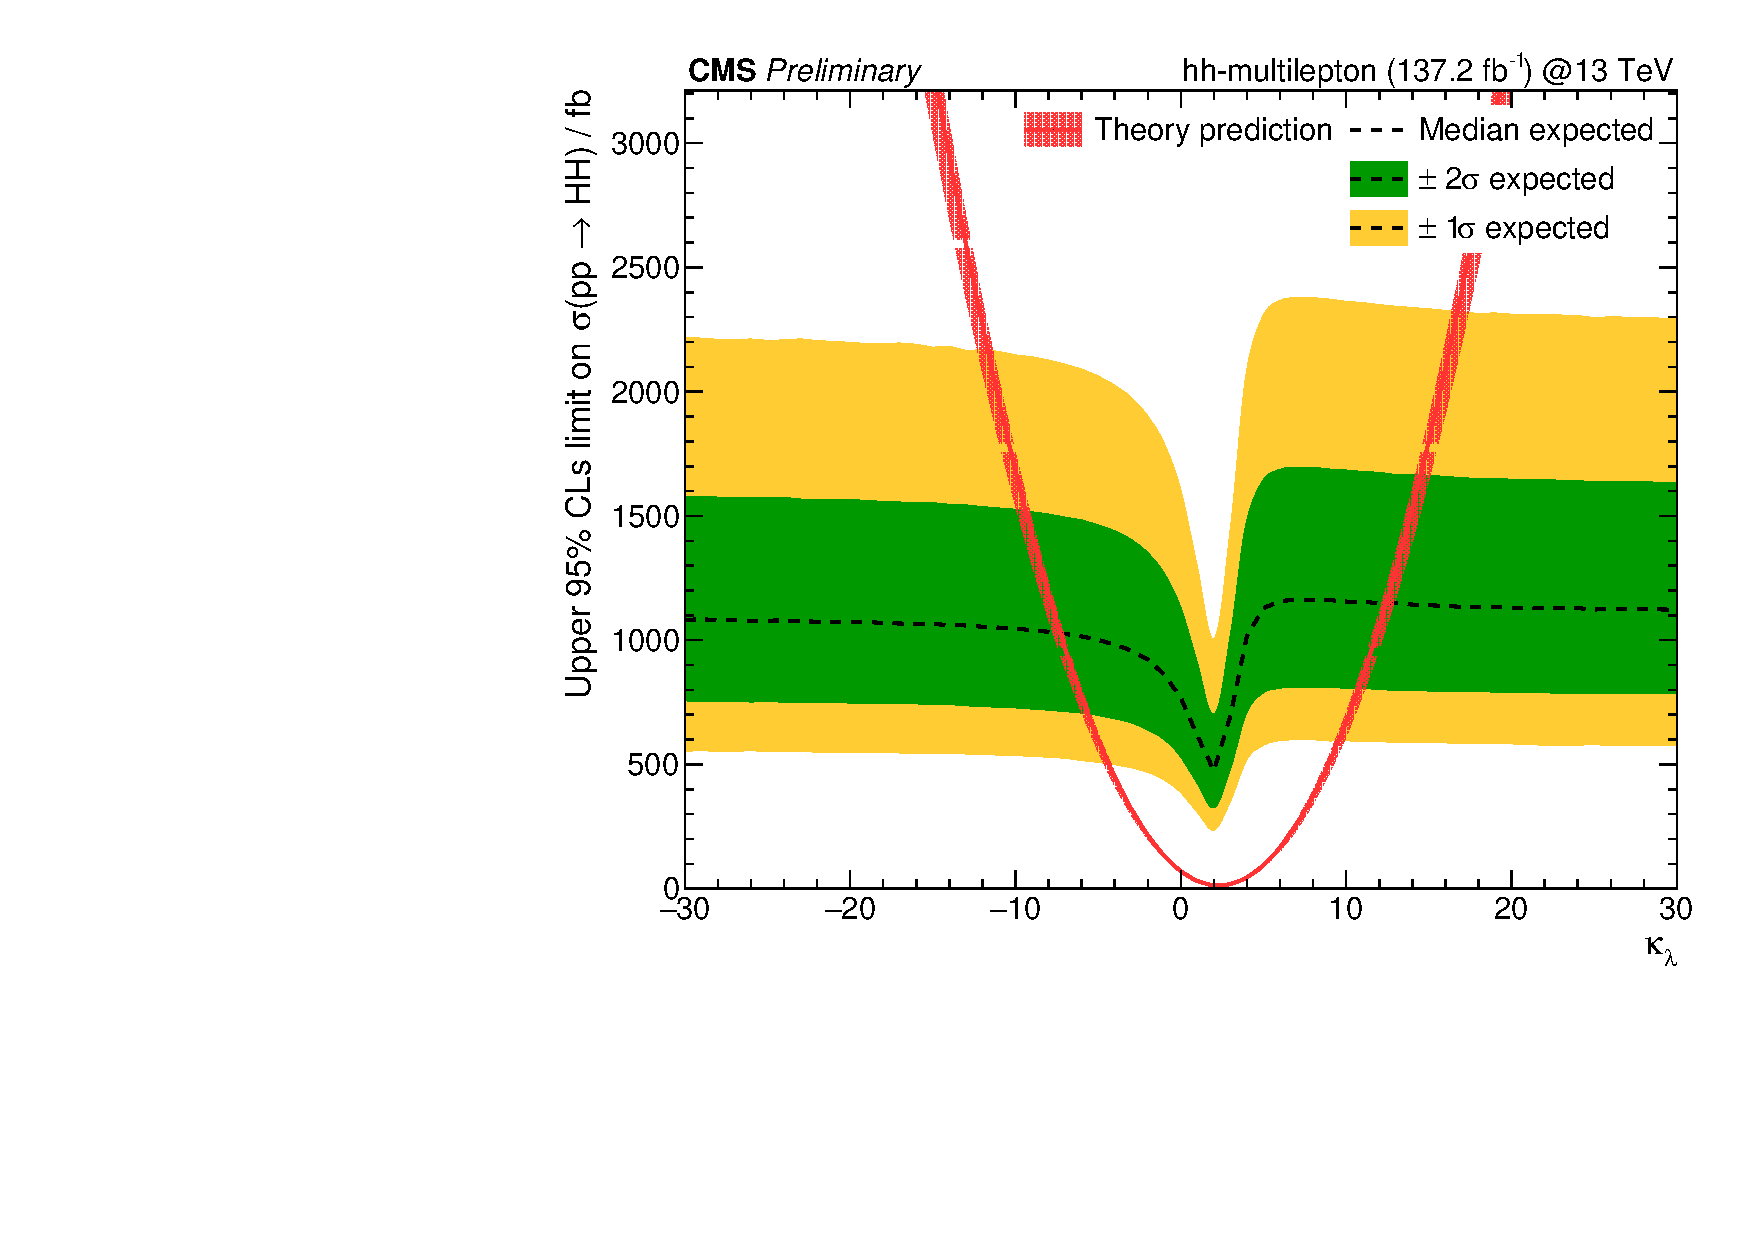
\includegraphics[width=0.45\textwidth]{figures/klscan.pdf}
  \hspace{0.05\textwidth}
  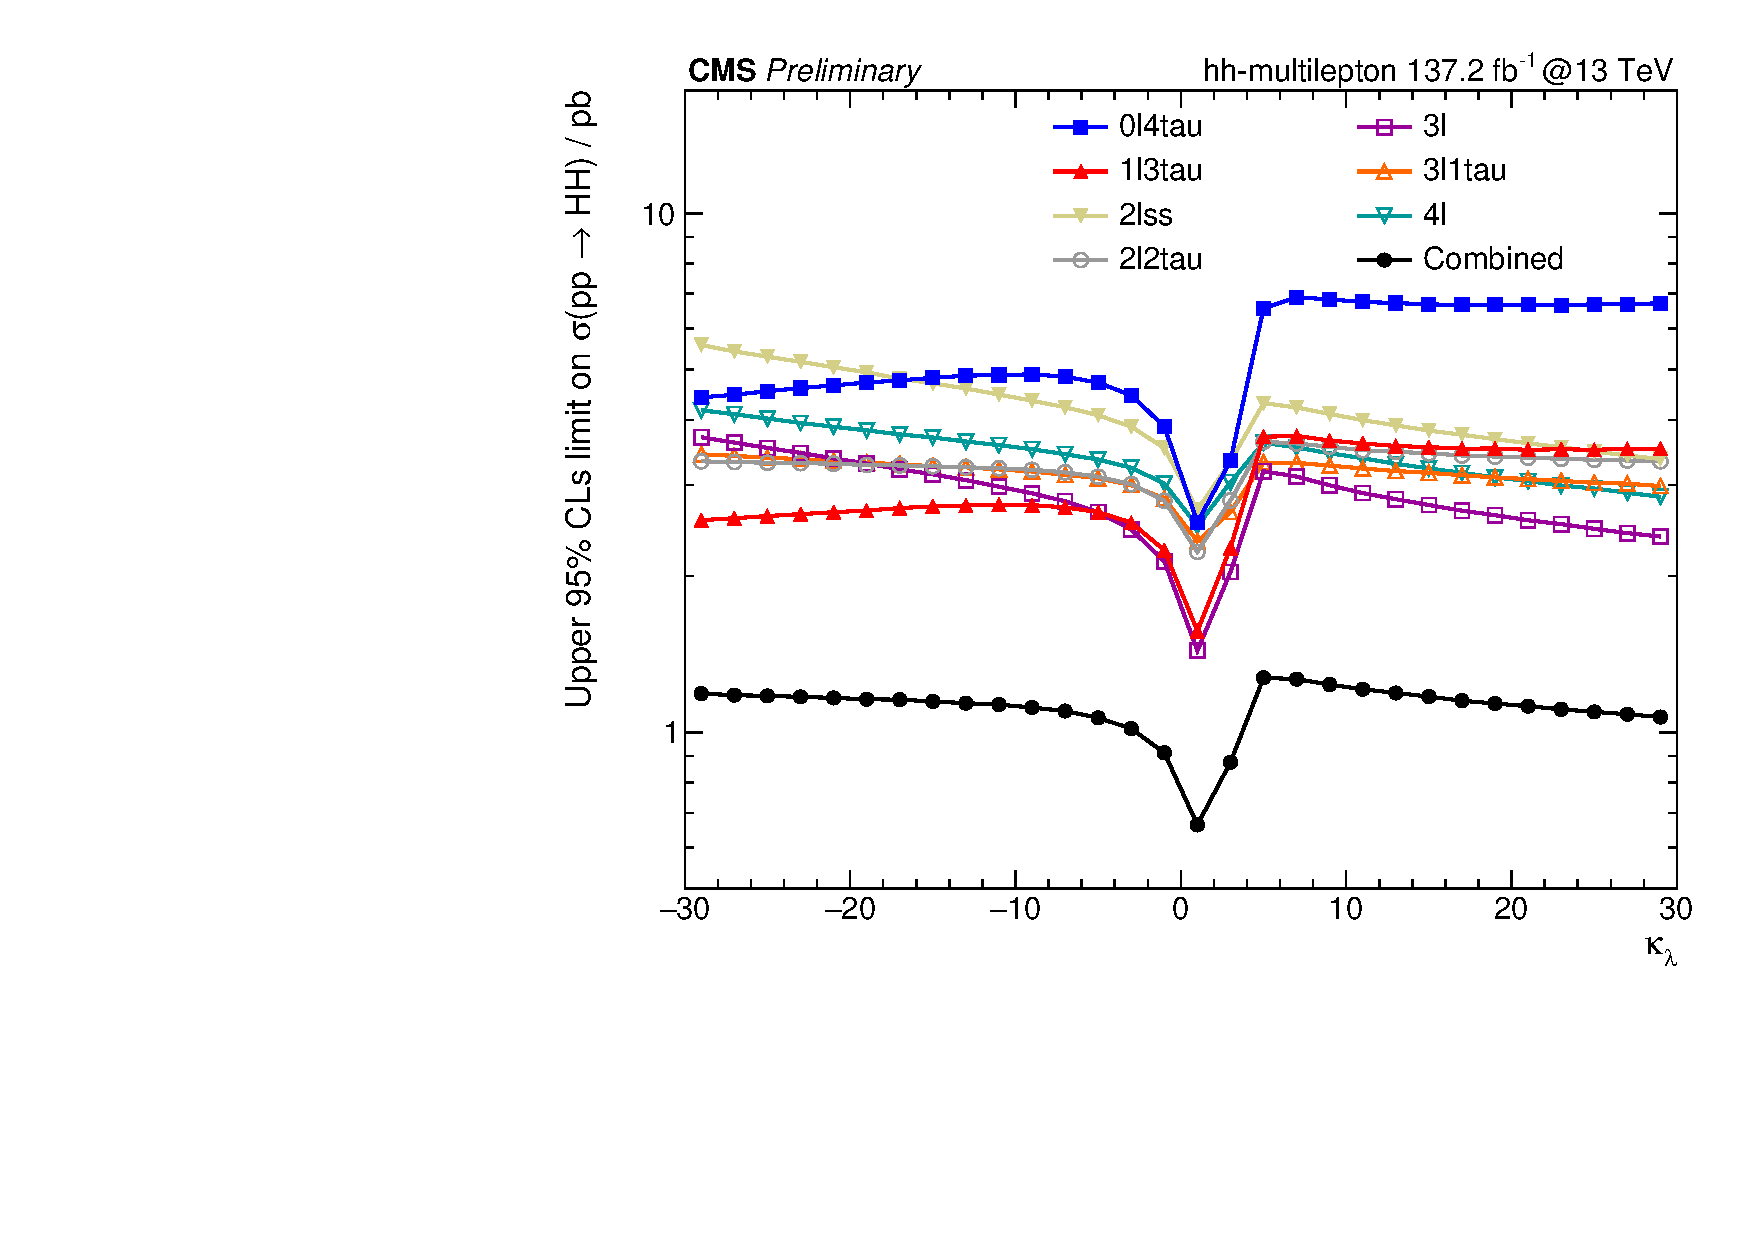
\includegraphics[width=0.45\textwidth]{figures/klMultiscan.pdf}
  \caption{
    Observed and expected 95\% CL limits on the $\HH$ production cross section as
    a function of the Higgs boson self-coupling strength modifier $\kappal$.
    The plot on the left shows the result obtained by combining all seven search categories,
    while the plot on the right shows the limits obtained for each search category separately.  Overlaid is a curve representing the
    predicted $\HH$ production cross section if all SM constants other than
    $\lambda$ have the values predicted in the SM.
  }
  \label{fig:HH_limits_kLambda}
\end{figure}

The observed and expected limits on the $\HH$ production cross section in the
twelve EFT benchmark scenarios are shown in Fig.~\ref{fig:HH_limits_EFT}
and summarized in Table~TODO.
For benchmarks X, Y, and Z, the upper limit cross sections are lower
than for any previous measurement~\cite{Sirunyan:2745738}.
These benchmarks represent models in which the $\HH$ invariant mass is
lower than the SM prediction.  This analysis has a higher signal efficiency
in the low-mass phase space compared to $\HH$ analyses performed in final states with bottom quarks,
because the reconstruction and identification efficiency for low-$\pt$ electrons and muons is higher than for jets of low $\pt$ in CMS.

\begin{figure}
  \centering
  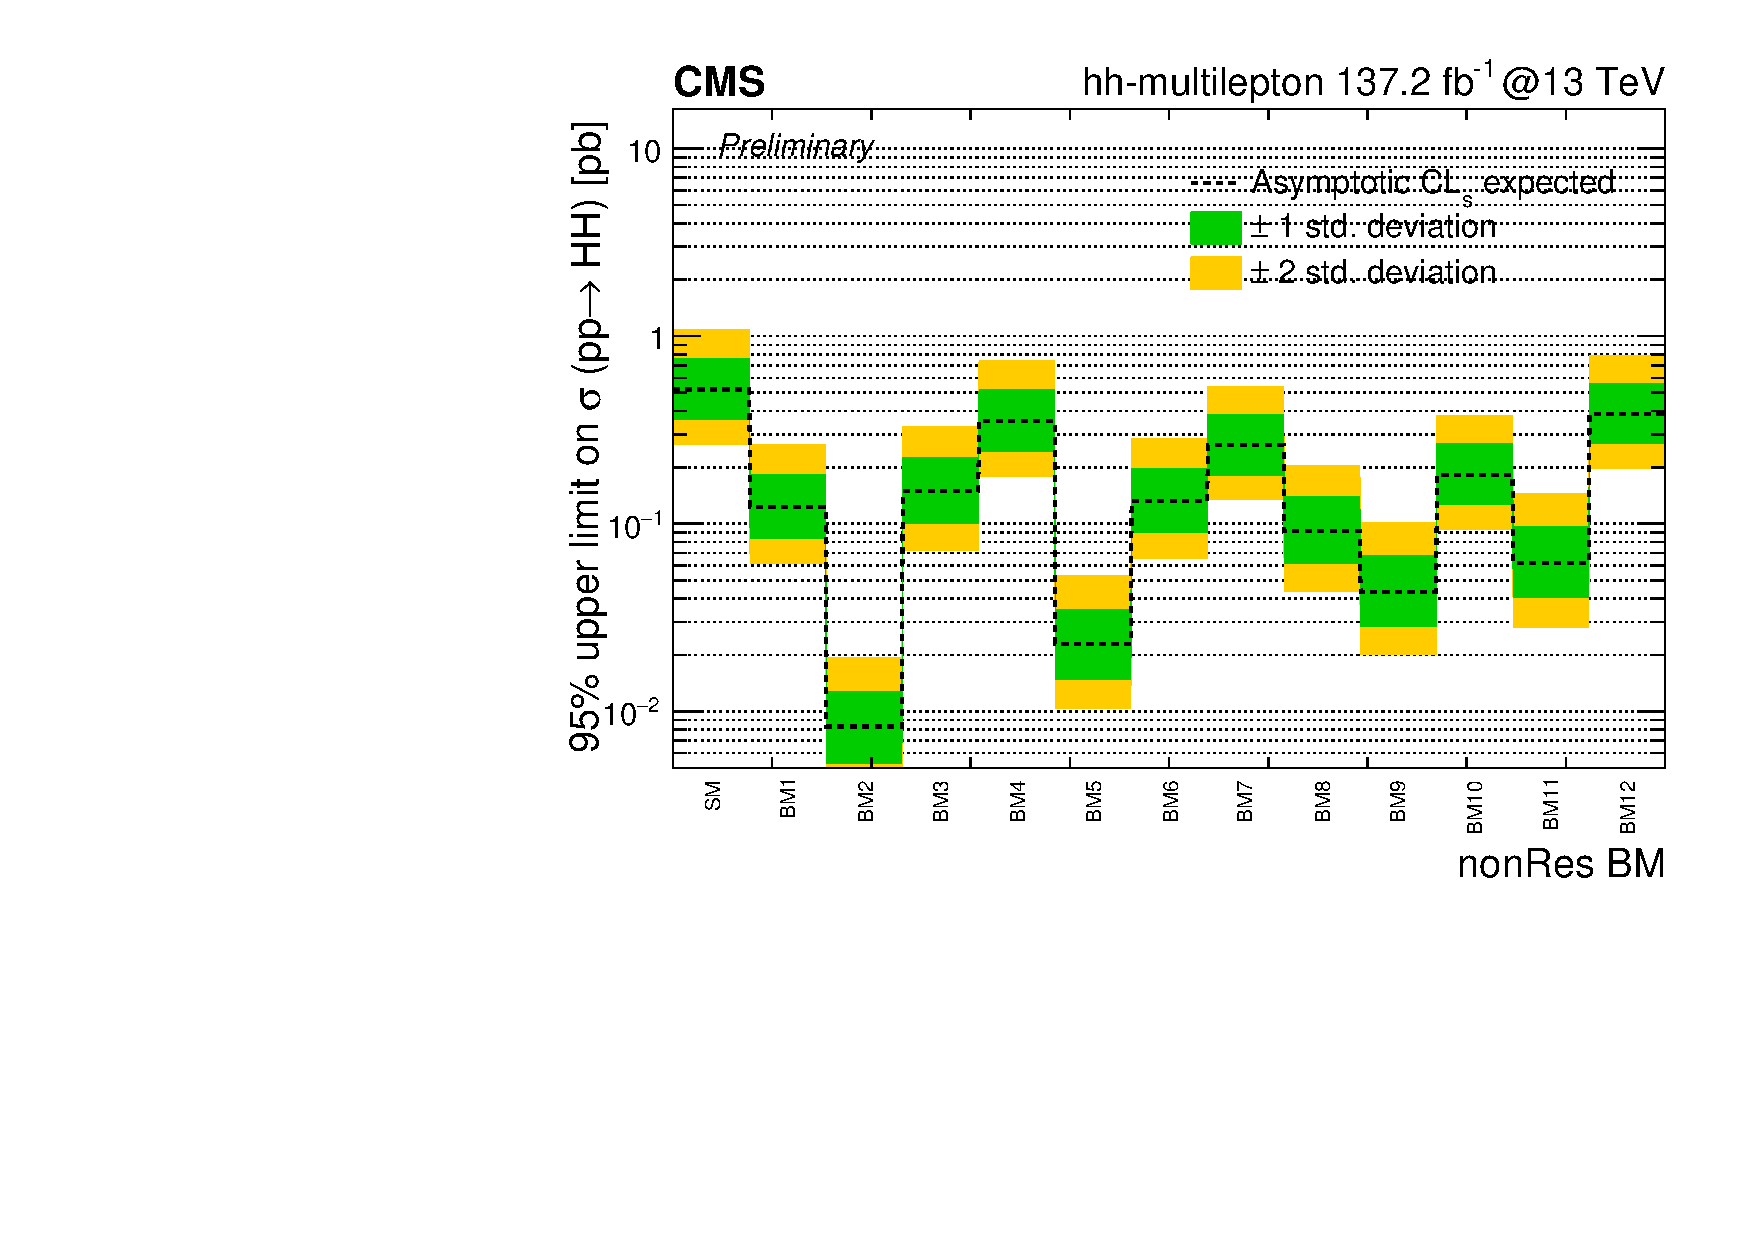
\includegraphics[width=0.45\textwidth]{figures/bmScan_multilepton_RUN2.pdf}
  \hspace{0.05\textwidth}
  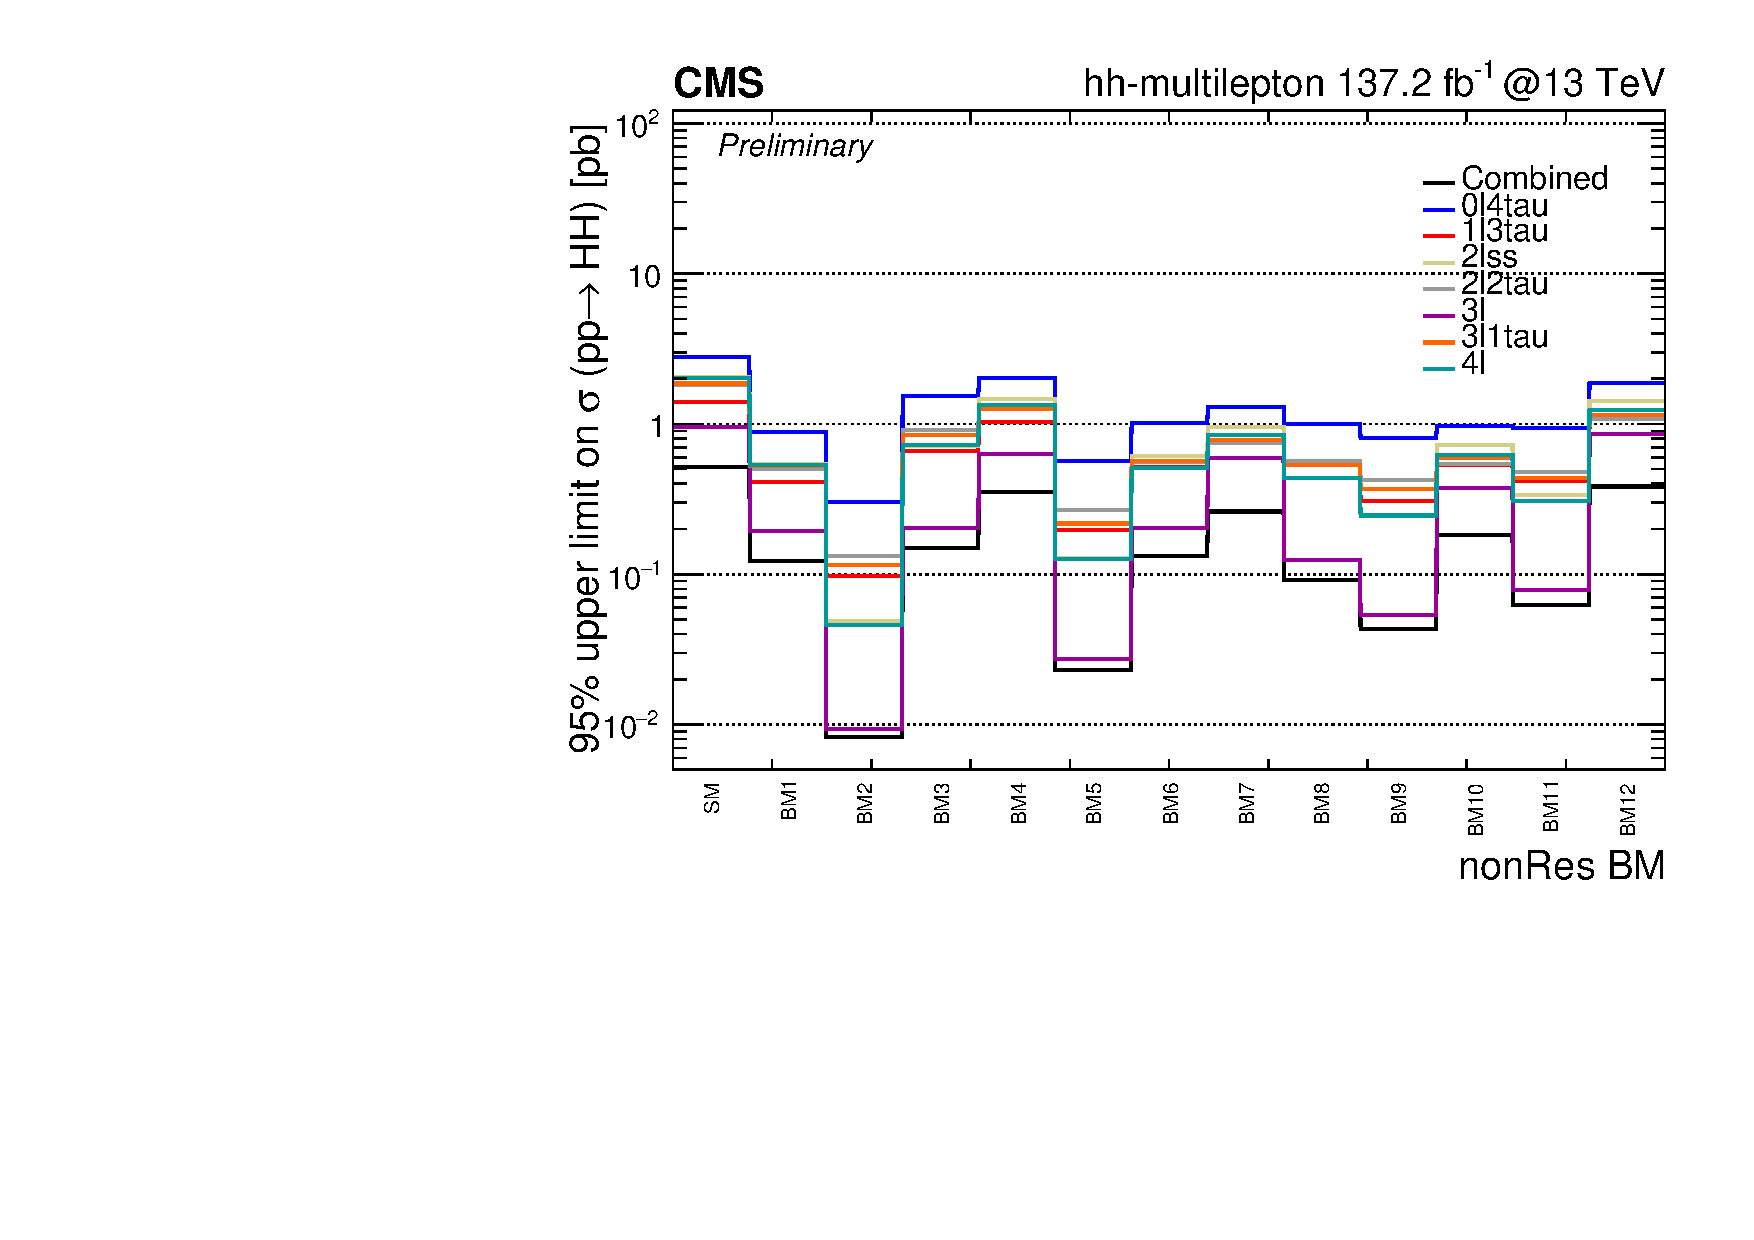
\includegraphics[width=0.45\textwidth]{figures/multiBMScan_multilepton_Run2.pdf}
  \caption{
    Observed and expected 95\% CL limits on the $\HH$ production cross section for
    twelve EFT benchmark scenarios and for the SM.
    The plot on the left shows the result obtained by combining all seven search categories,
    while the plot on the right shows the limits obtained for each search category separately. 
  }
  \label{fig:HH_limits_EFT}
\end{figure}

Figures~\ref{fig:HH_limits_spin0} and \ref{fig:HH_limits_spin2} show the observed and
expected limits on the resonant $\HH$ production cross section as a function of the mass $m_{\X}$ of the particle $\X$,
for spin-0 and spin-2 particles decaying to a $\PHiggs$ boson pair.
Compared to previously published searches for resonant $\HH$
production~\cite{Sirunyan:2018ayu,2020135103},
this analysis has similar sensitivity at very low masses ($250$-$400\GeV$),
owing again to the efficient reconstruction and identification of low-$\pt$ leptons in CMS.

\begin{figure}
  \centering
  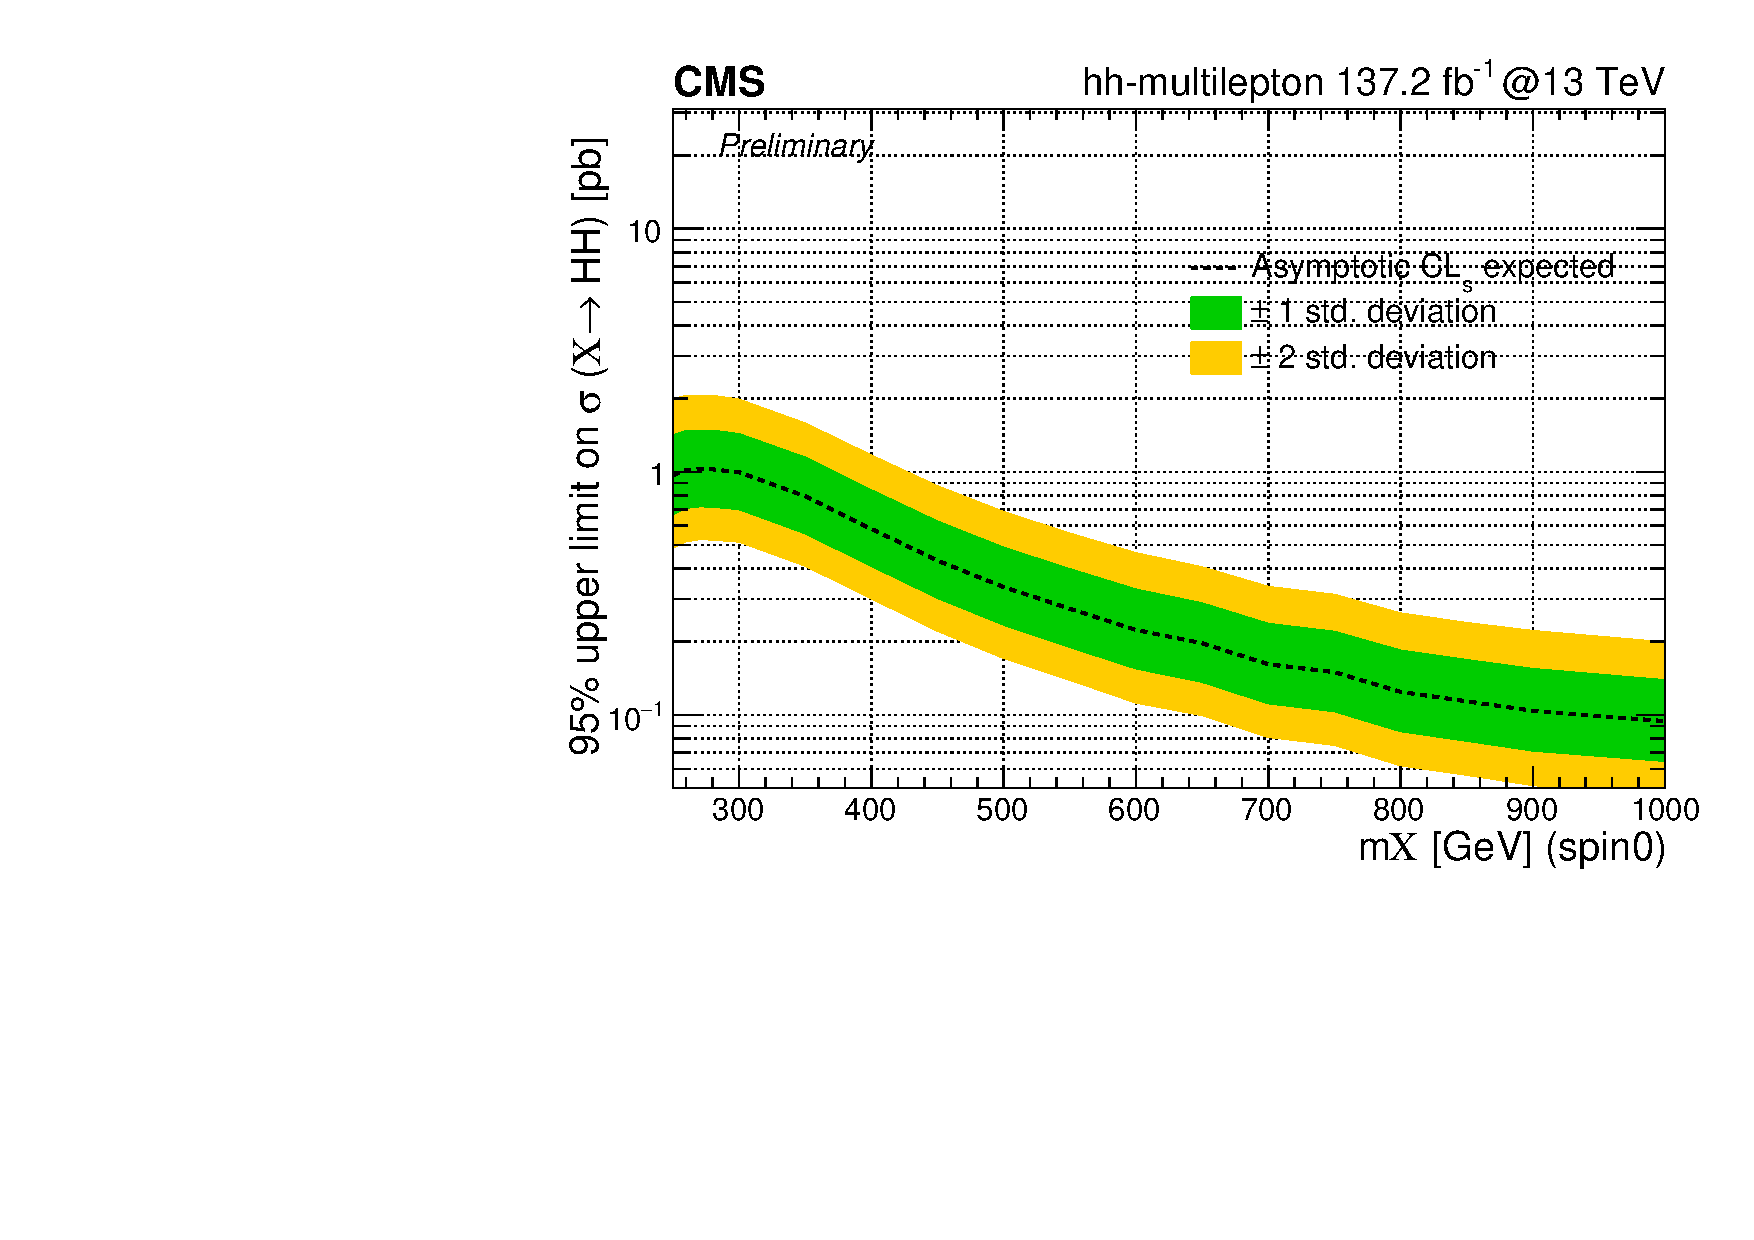
\includegraphics[width=0.45\textwidth]{figures/massScan_spin0_multilepton_RUN2.pdf}
  \hspace{0.05\textwidth}
  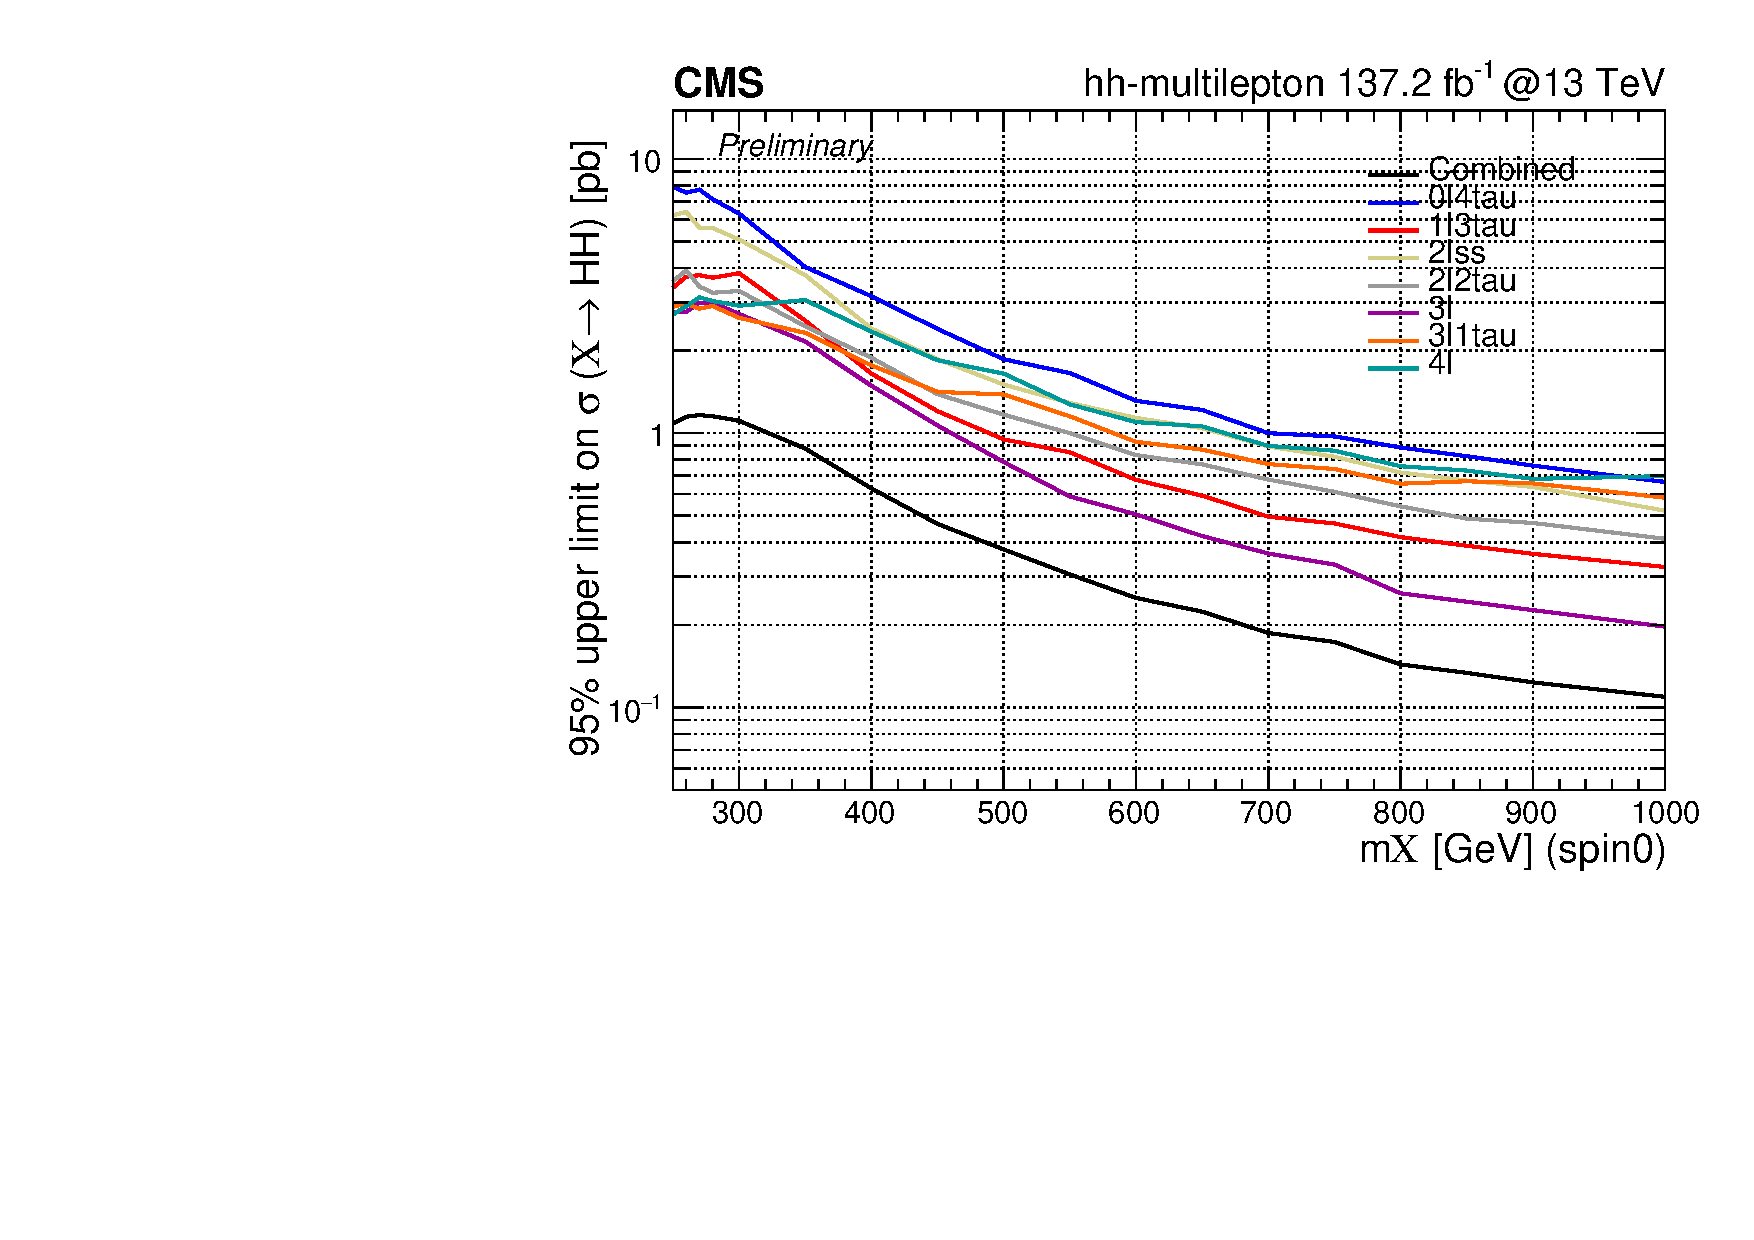
\includegraphics[width=0.45\textwidth]{figures/massMultiScan_spin0_multilepton_Run2.pdf}
  \caption{
    Observed and expected 95\% CL limits on the production of new particles $\X$ of spin $0$ 
    and mass $m_{\X}$ in the range $250 \leq m_{\X} \leq 1000\GeV$, which decay to $\PHiggs$ boson pairs,
    for the combination of all seven search categories (left)
    and for each search category separately (right).
  }
  \label{fig:HH_limits_spin0}
\end{figure}

\begin{figure}
  \centering
  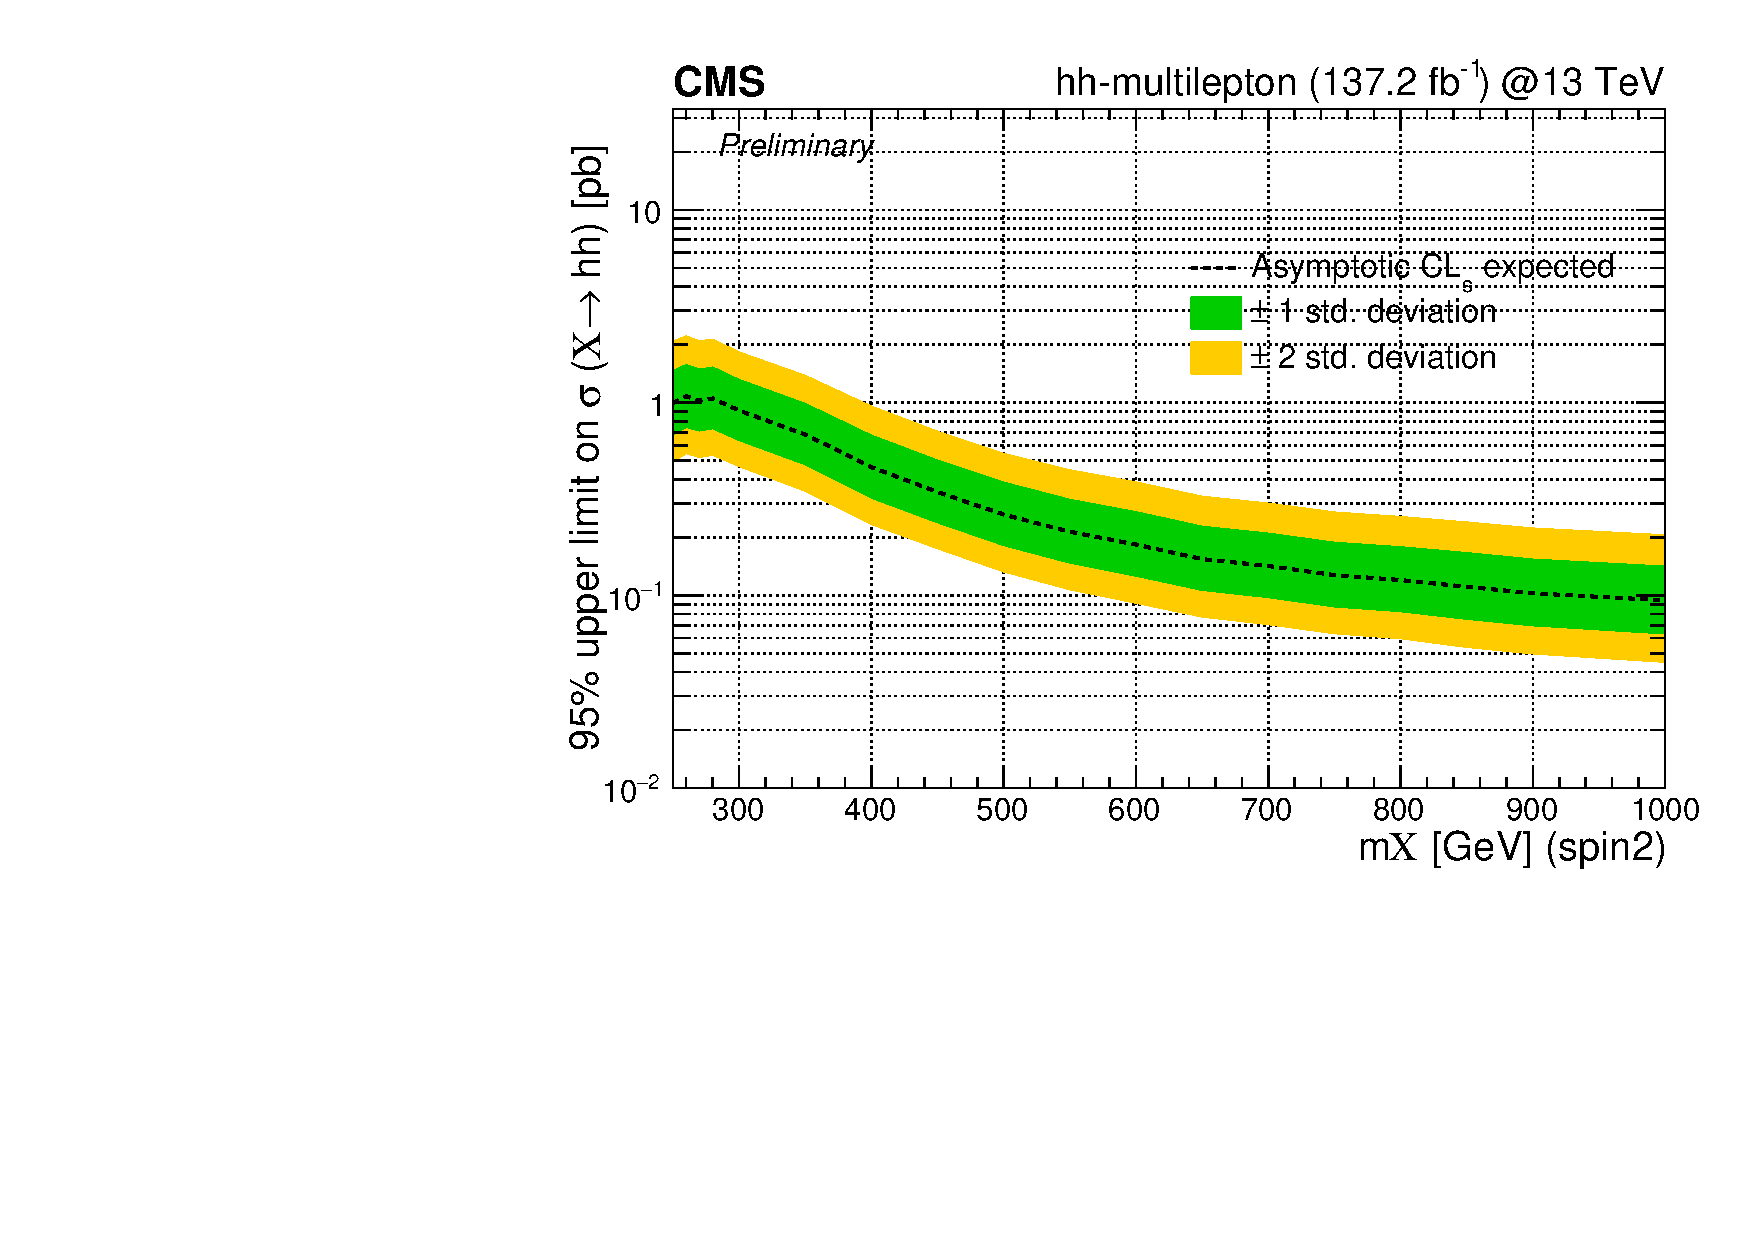
\includegraphics[width=0.45\textwidth]{figures/massScan_spin2_multilepton_RUN2.pdf}
  \hspace{0.05\textwidth}
  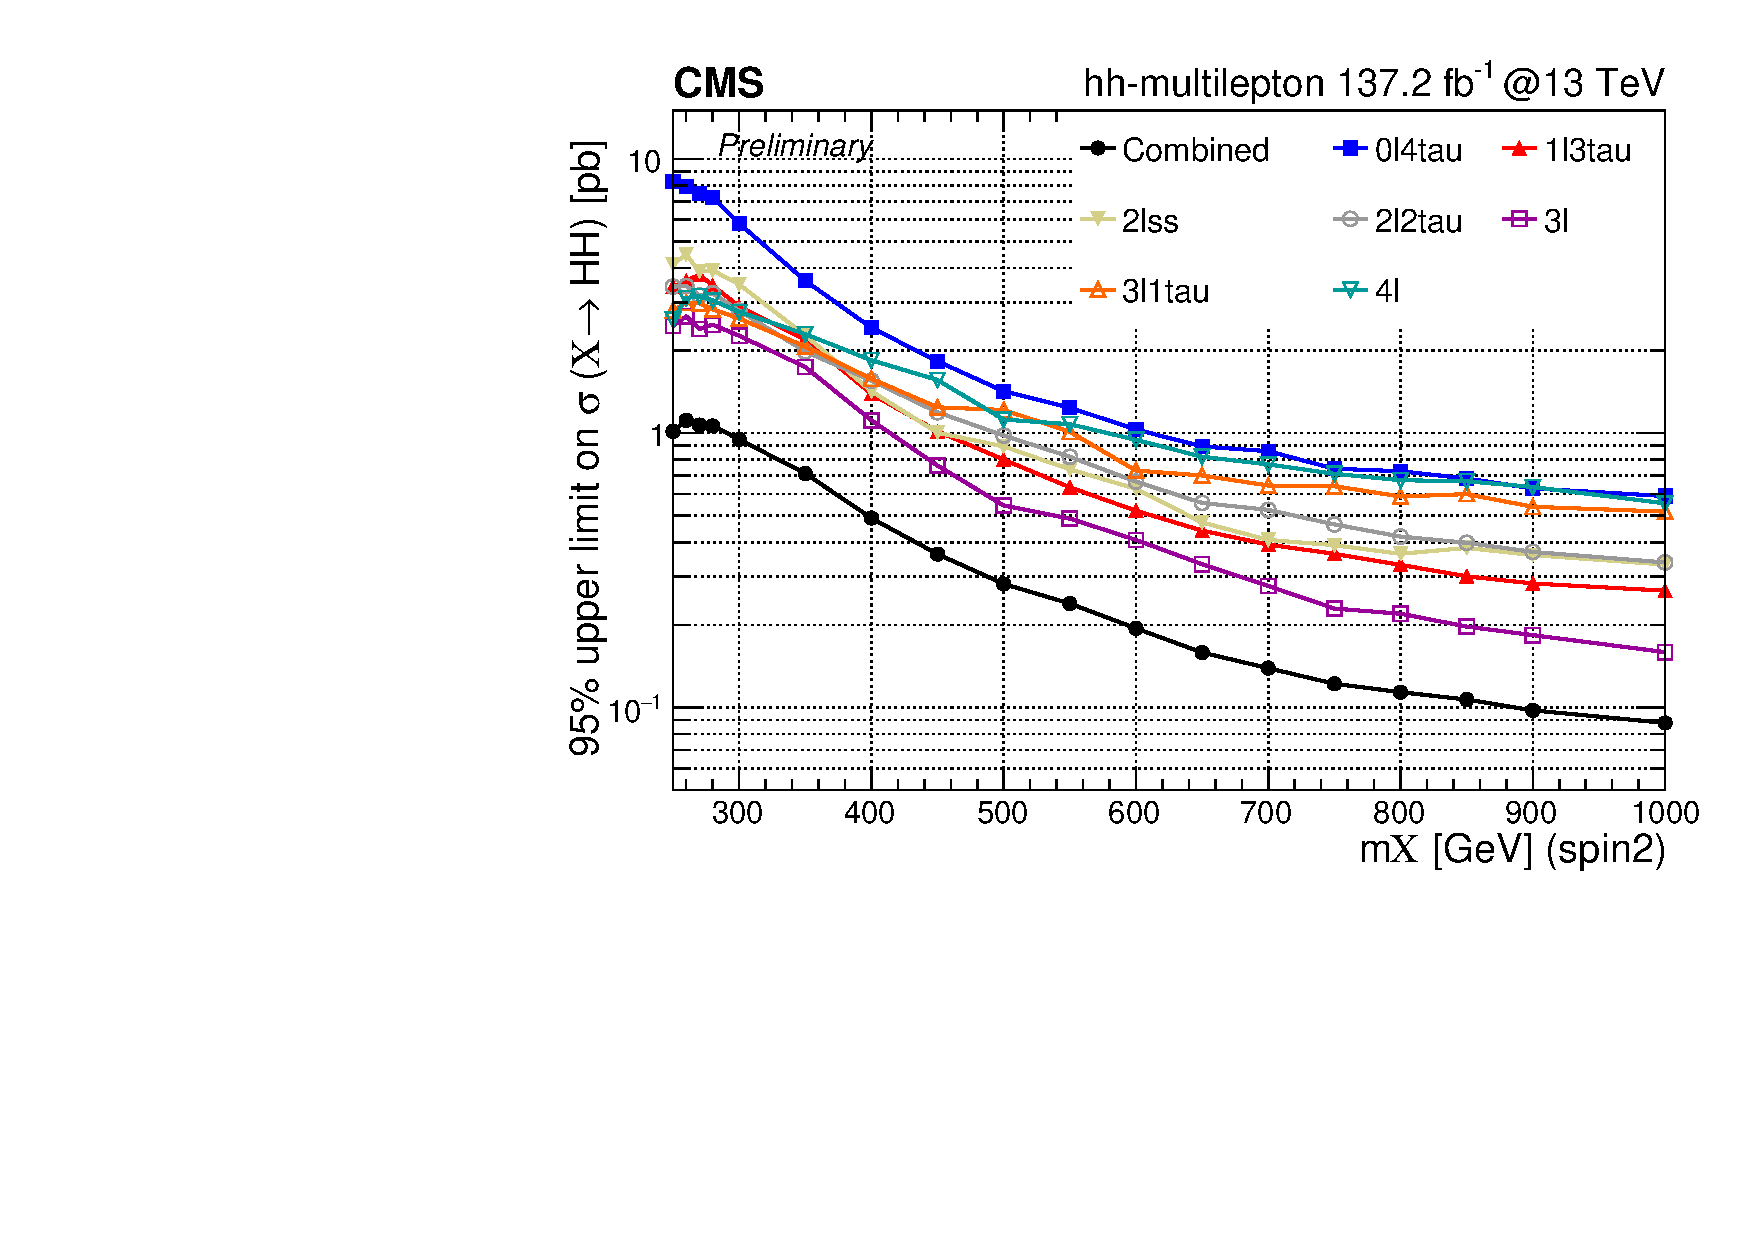
\includegraphics[width=0.45\textwidth]{figures/massMultiScan_spin2_multilepton_Run2.pdf}
  \caption{
    Observed and expected 95\% CL limits on the production of new particles $\X$ of spin $2$ 
    and mass $m_{\X}$ in the range $250 \leq m_{\X} \leq 1000\GeV$, which decay to $\PHiggs$ boson pairs,
    for the combination of all seven search categories (left)
    and for each search category separately (right).
  }
  \label{fig:HH_limits_spin2}
\end{figure}
